
\begin{appendices} 	% starts appendix
\addtocontents{toc}{\protect\setcounter{tocdepth}{1}} % 
\makeatletter
\addtocontents{toc}{%
  \begingroup
  \let\protect\l@chapter\protect\l@section
  \let\protect\l@section\protect\l@subsection
}
\makeatother

%********* RECTIFIER appendix *********
\chapter{Rectifier Implementation}

\begin{figure} [!htbp]	% schematic Rectifier
 	\centering
  	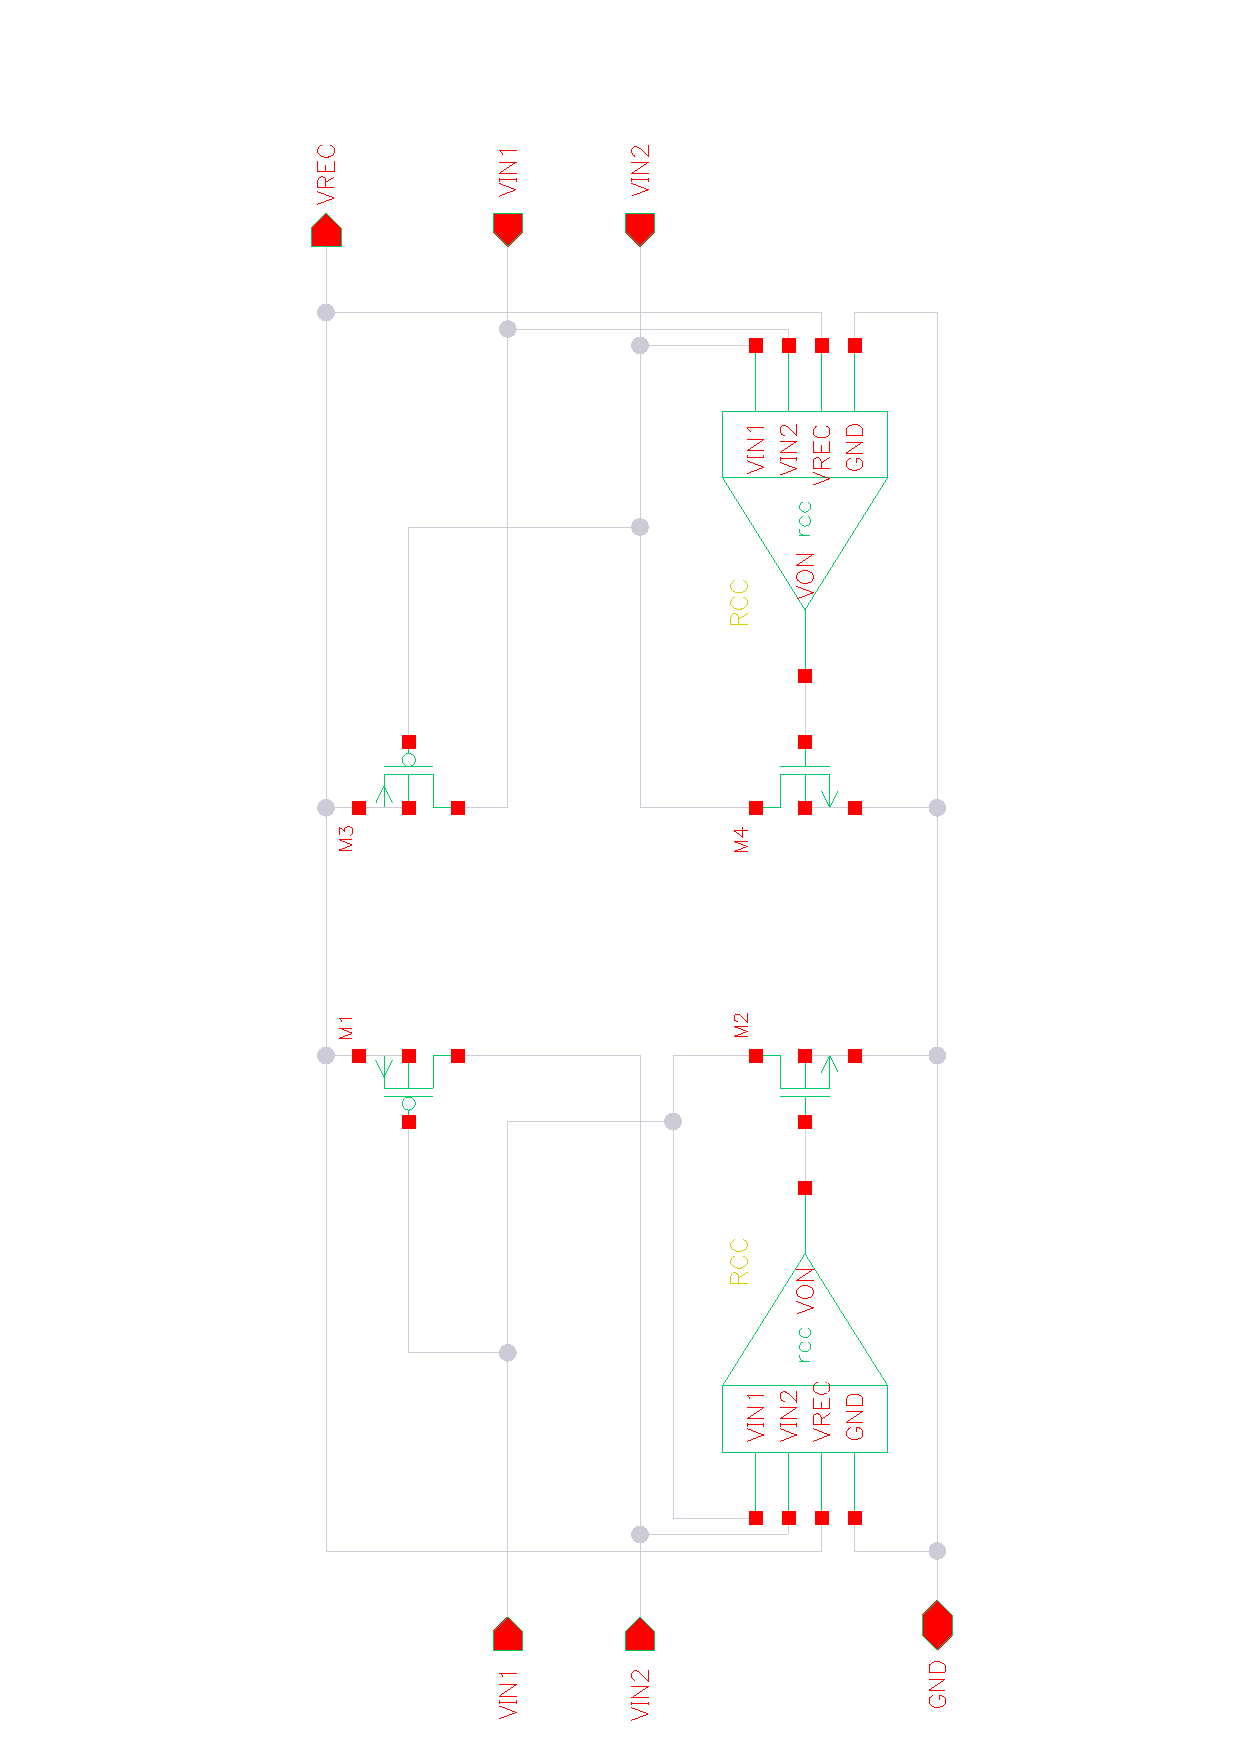
\includegraphics[width=\textwidth]{appendix/schematic_rectifier_l.pdf} 
 	\caption{Schematic of Rectifier} 
	\label{fig:appen_schematic_rectifer} 
\end{figure}

\begin{figure} [!htbp]	% schematic RCC
 	\centering
  	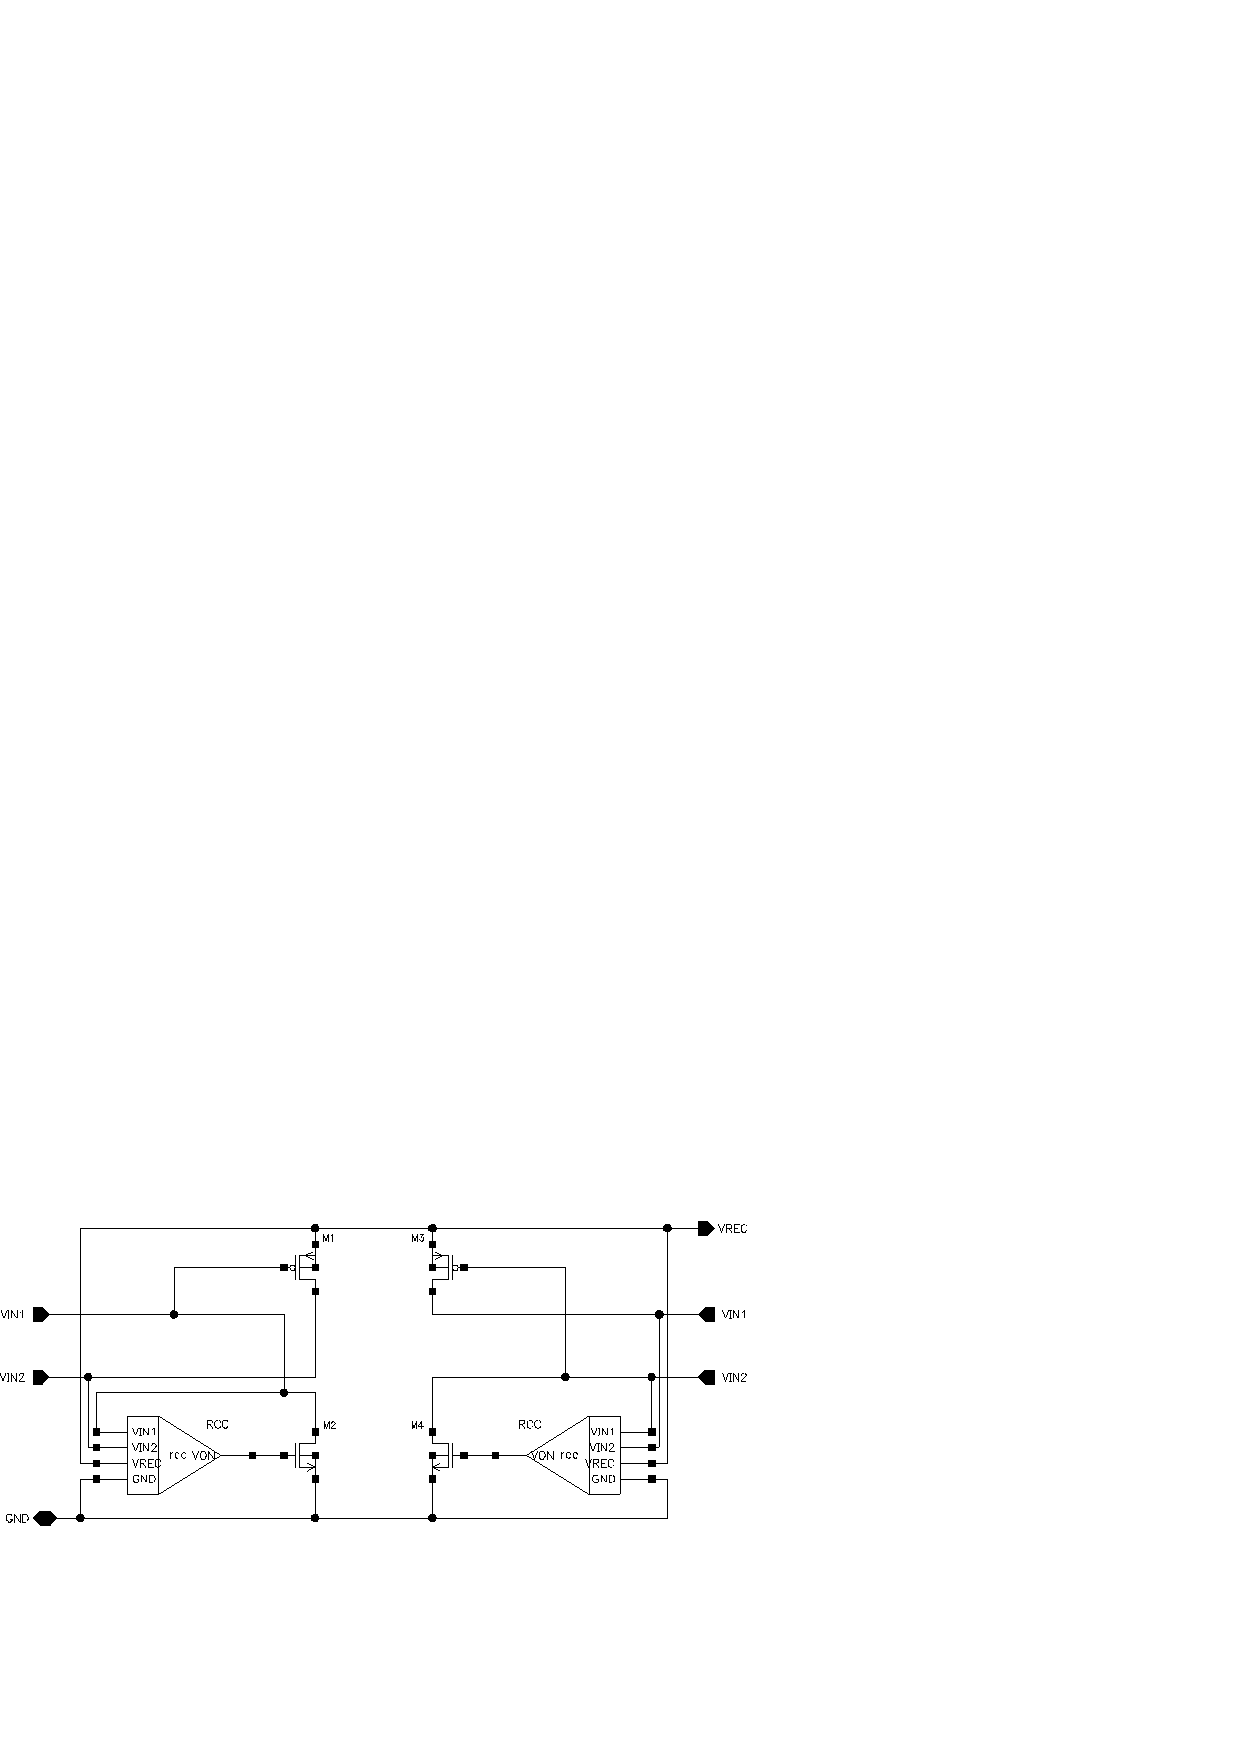
\includegraphics[width=\textwidth]{appendix/schematic_rectifier_bw.pdf} 
 	\caption{Schematic of RCC} 
	\label{fig:appen_schematic_rcc} 
\end{figure}

\begin{sidewaysfigure} [!htbp] % Layout Rectifer
 	\centering
  	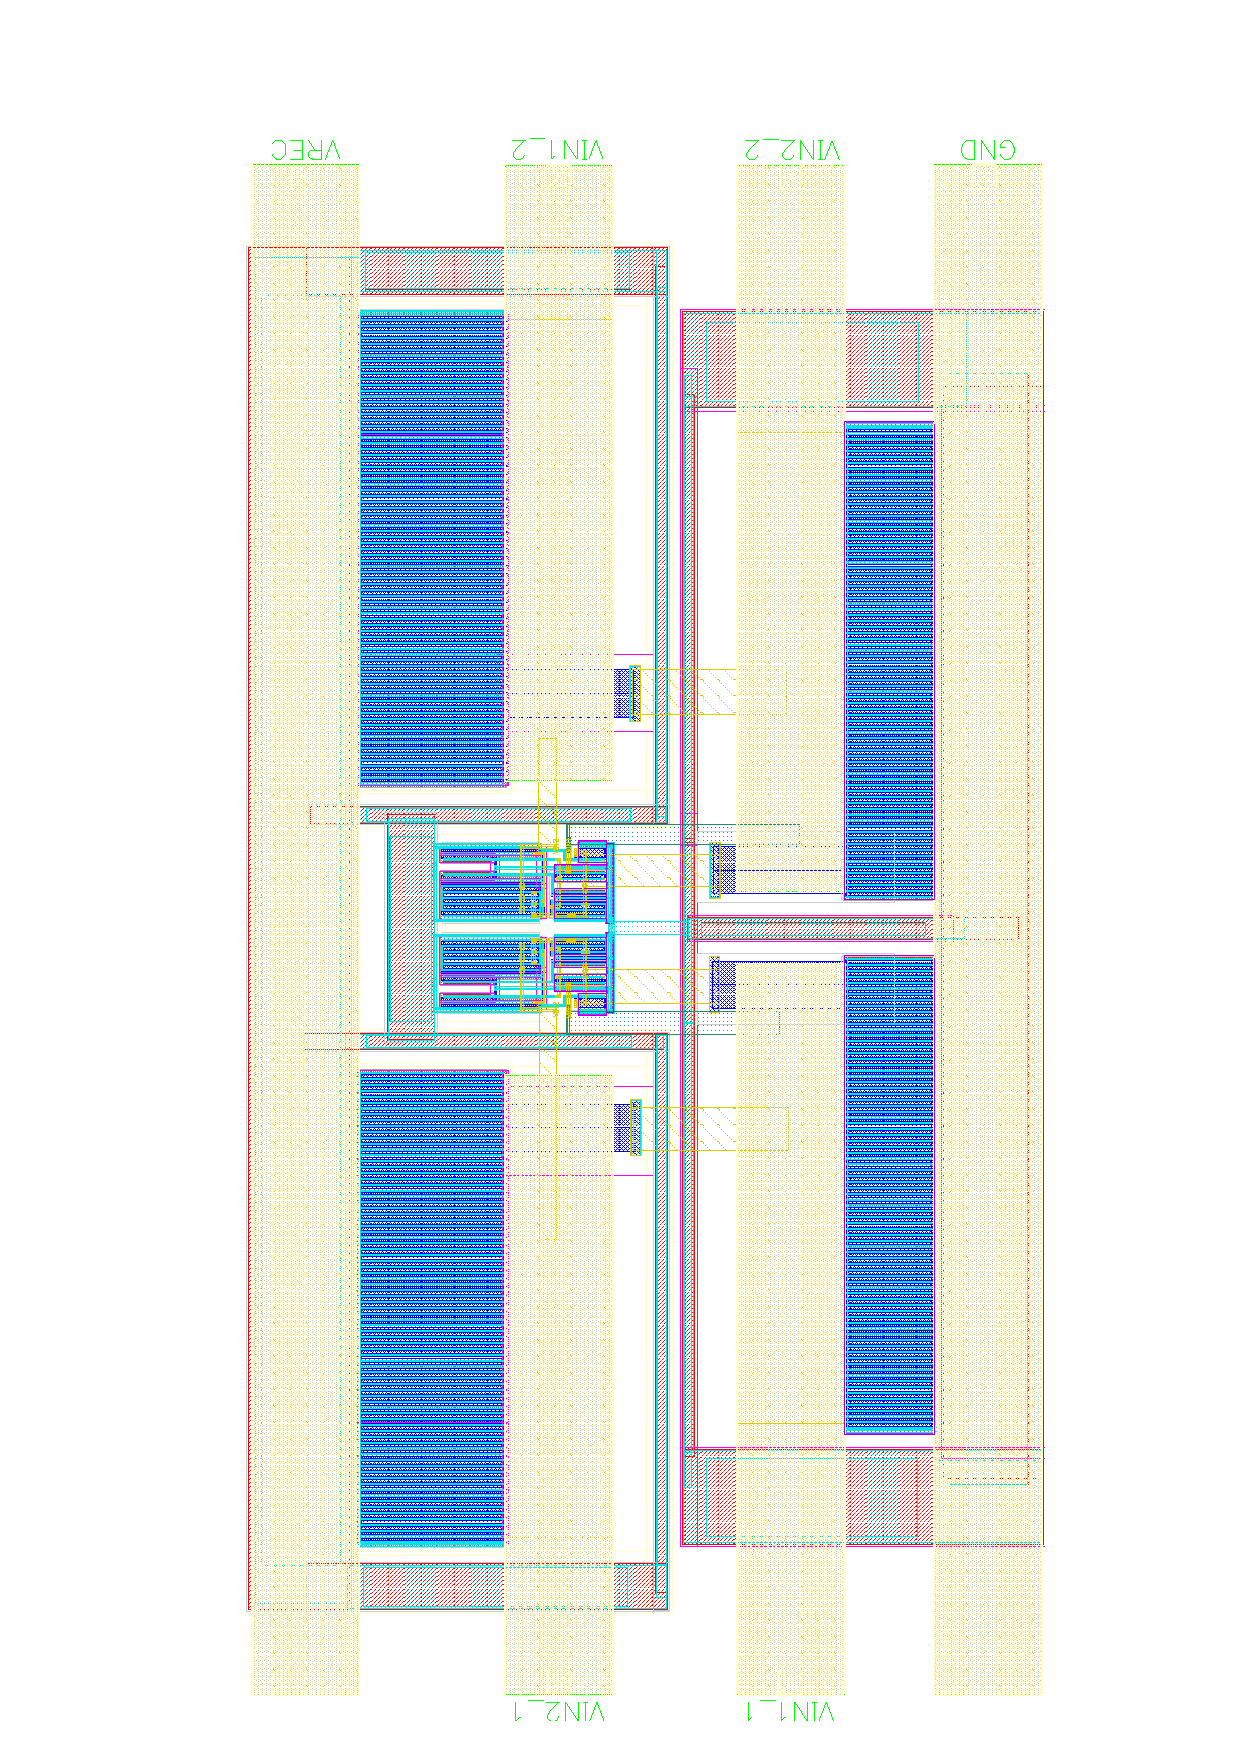
\includegraphics[width=\textwidth]{appendix/layout_rectifier_l.pdf} 
 	\caption{Layout of Rectifier} 
	\label{fig:appen_layout_rectifer} 
\end{sidewaysfigure}


%********* LDO appendix *********
\chapter{LDO Implementation}

\begin{figure} [!htbp]	% schematic LDO
 	\centering
  	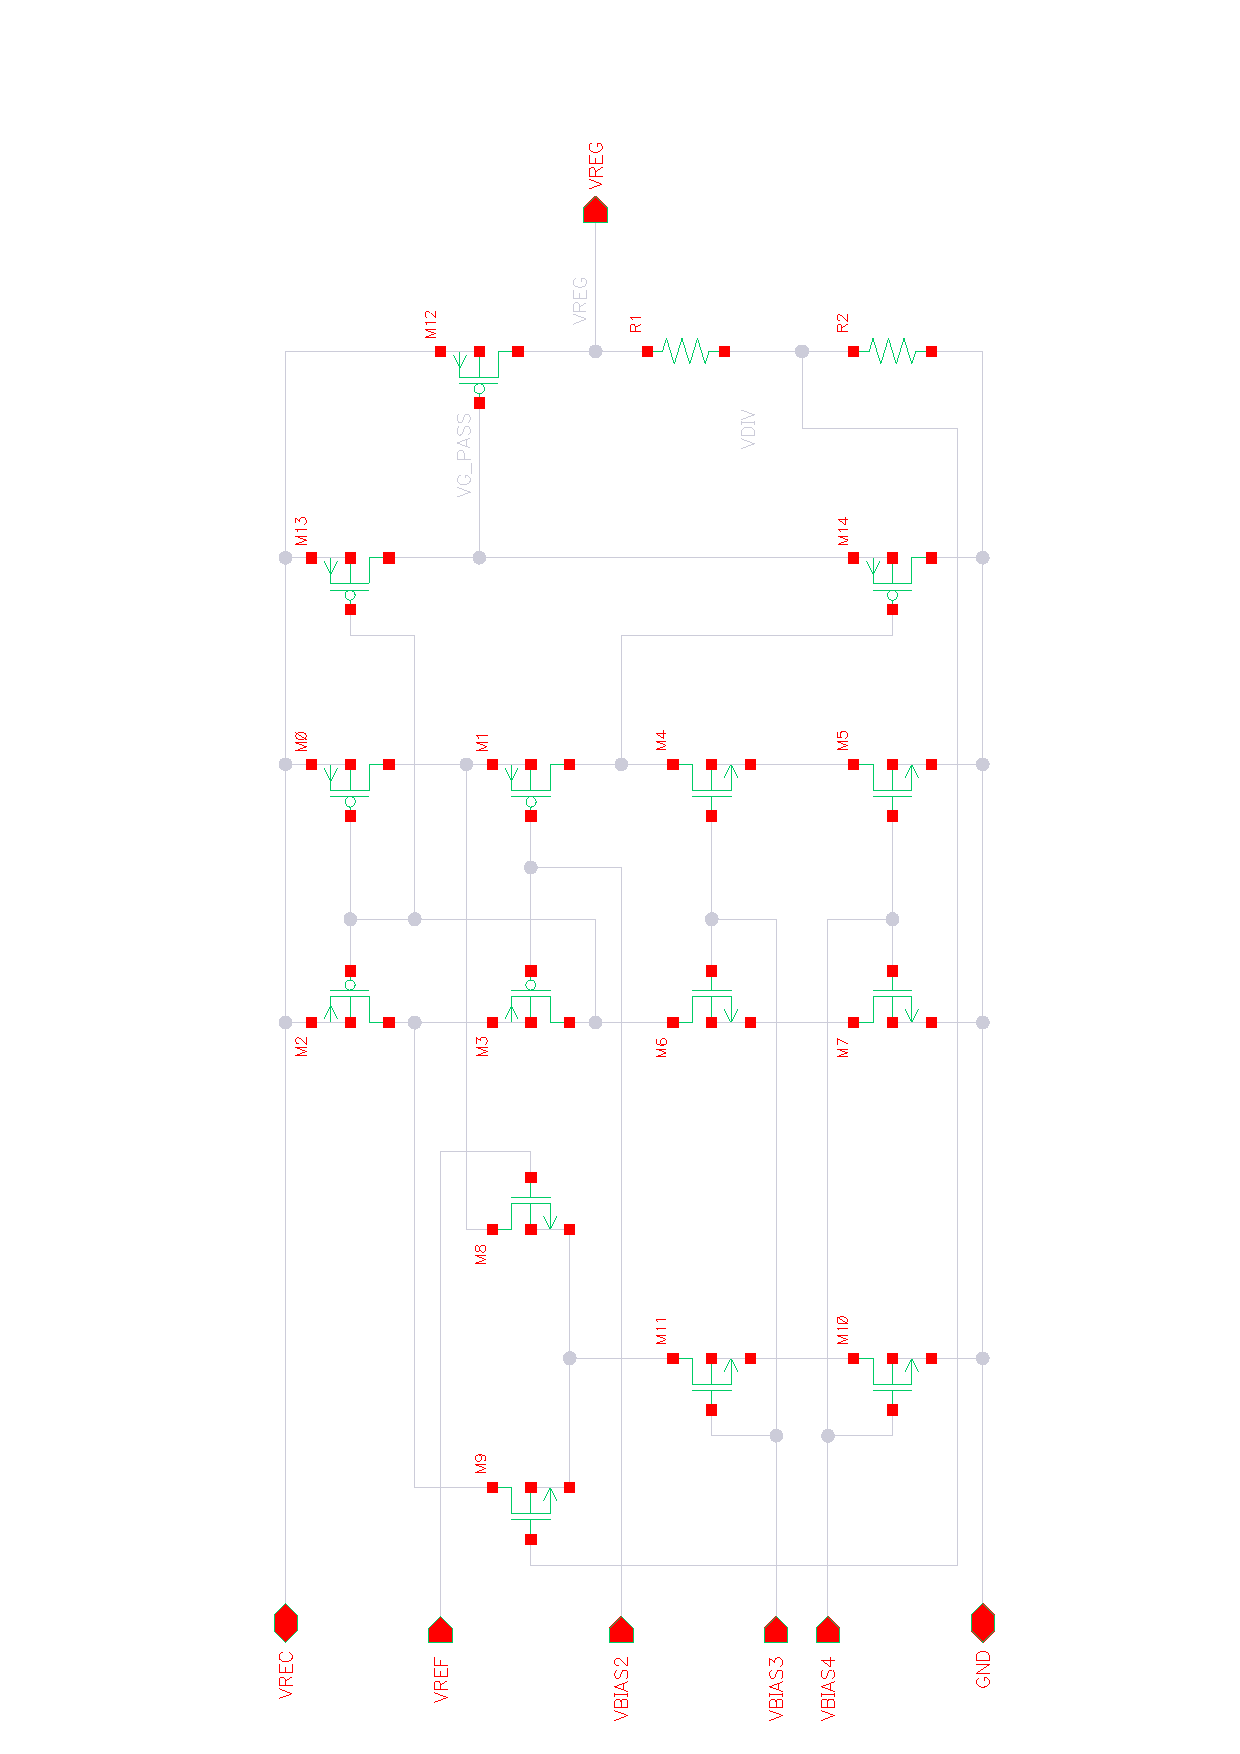
\includegraphics[angle=90, width=0.57\textwidth]{appendix/schematic_ldo_l.pdf} 
 	\caption{Schematic of LDO} 
	\label{fig:appen_schematic_ldo} 
\end{figure}

\begin{sidewaysfigure} [!htbp]	% Layout LDO
 	\centering
  	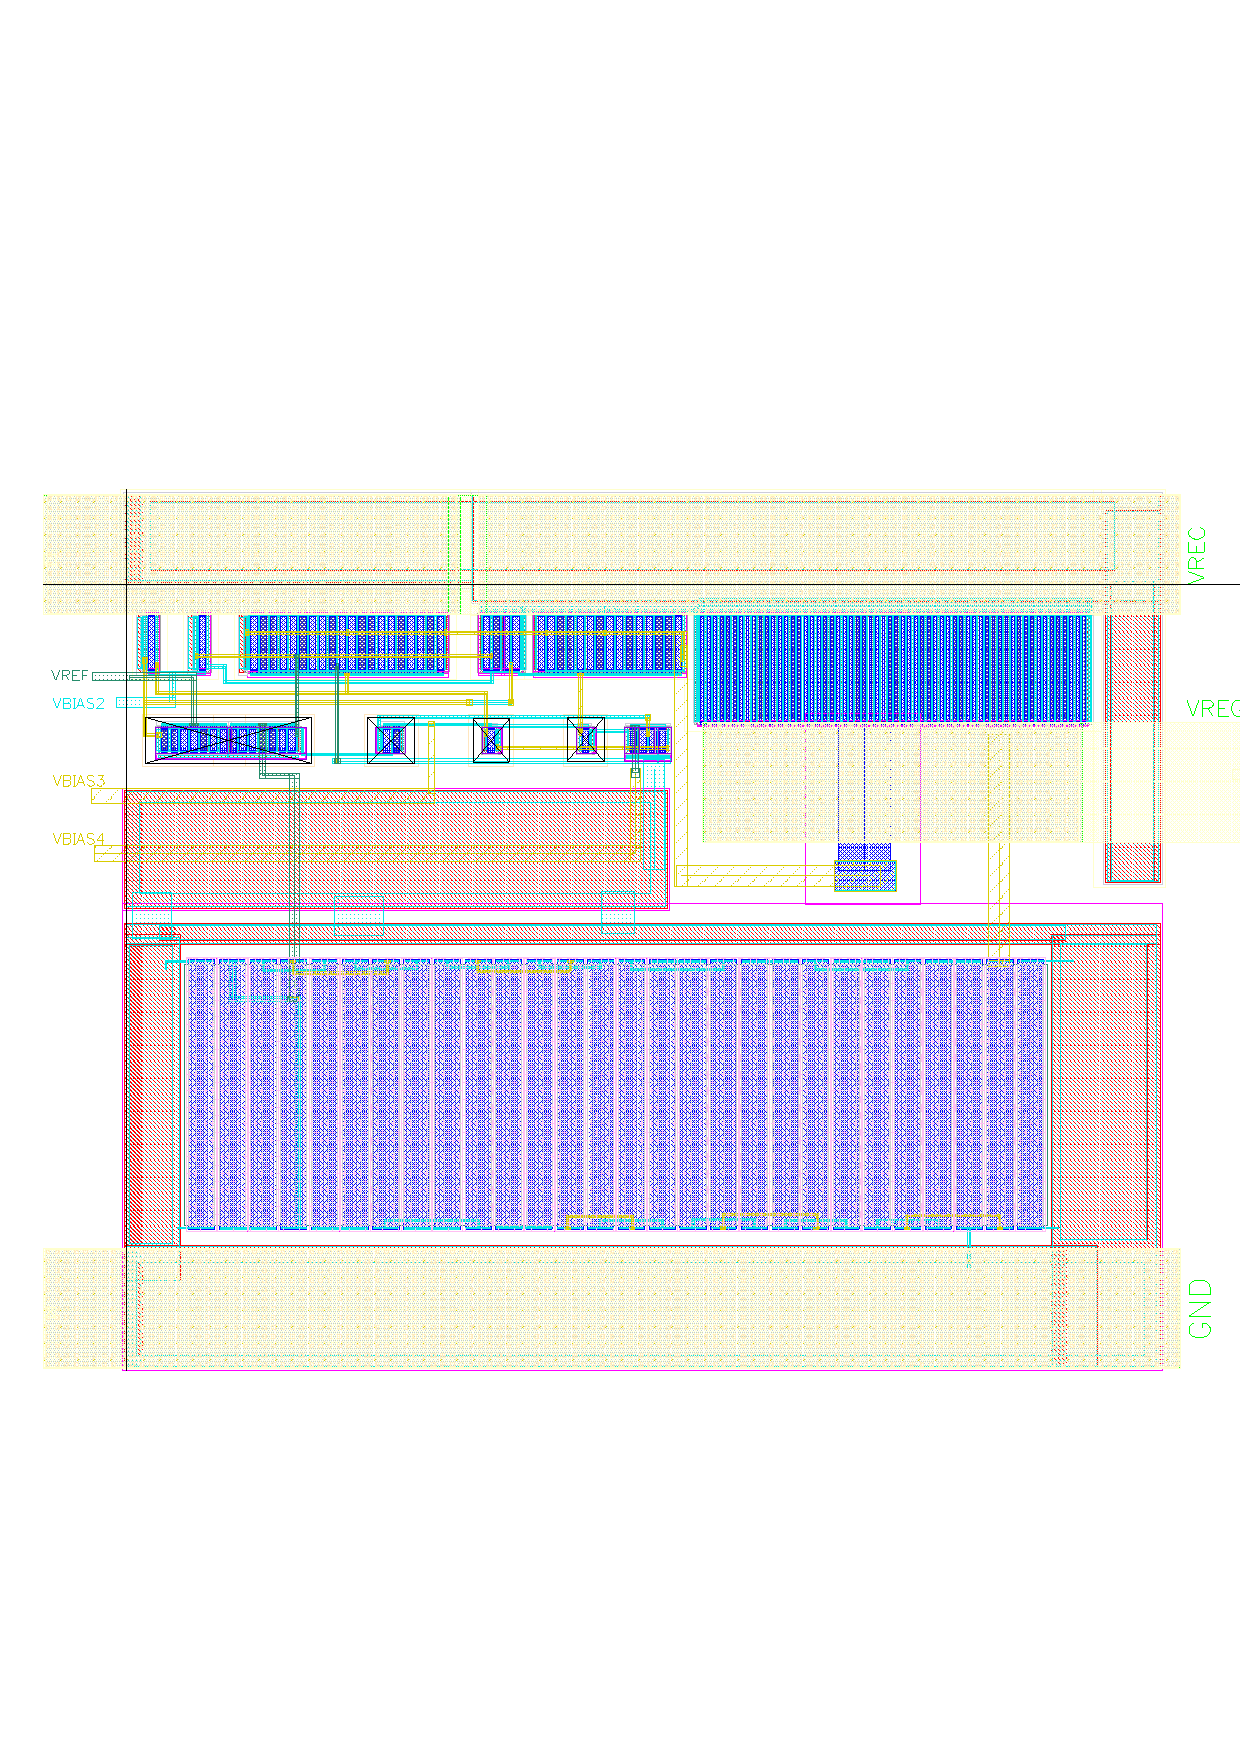
\includegraphics[width=0.77\textwidth]{appendix/layout_ldo_p.pdf} 
 	\caption{Layout of LDO} 
	\label{fig:appen_layout_ldo} 
\end{sidewaysfigure}


% ********* WPT appendix *********


\chapter{WPT Chip}

\begin{figure} [!htbp]	% schematic WPT top
 	\centering
  	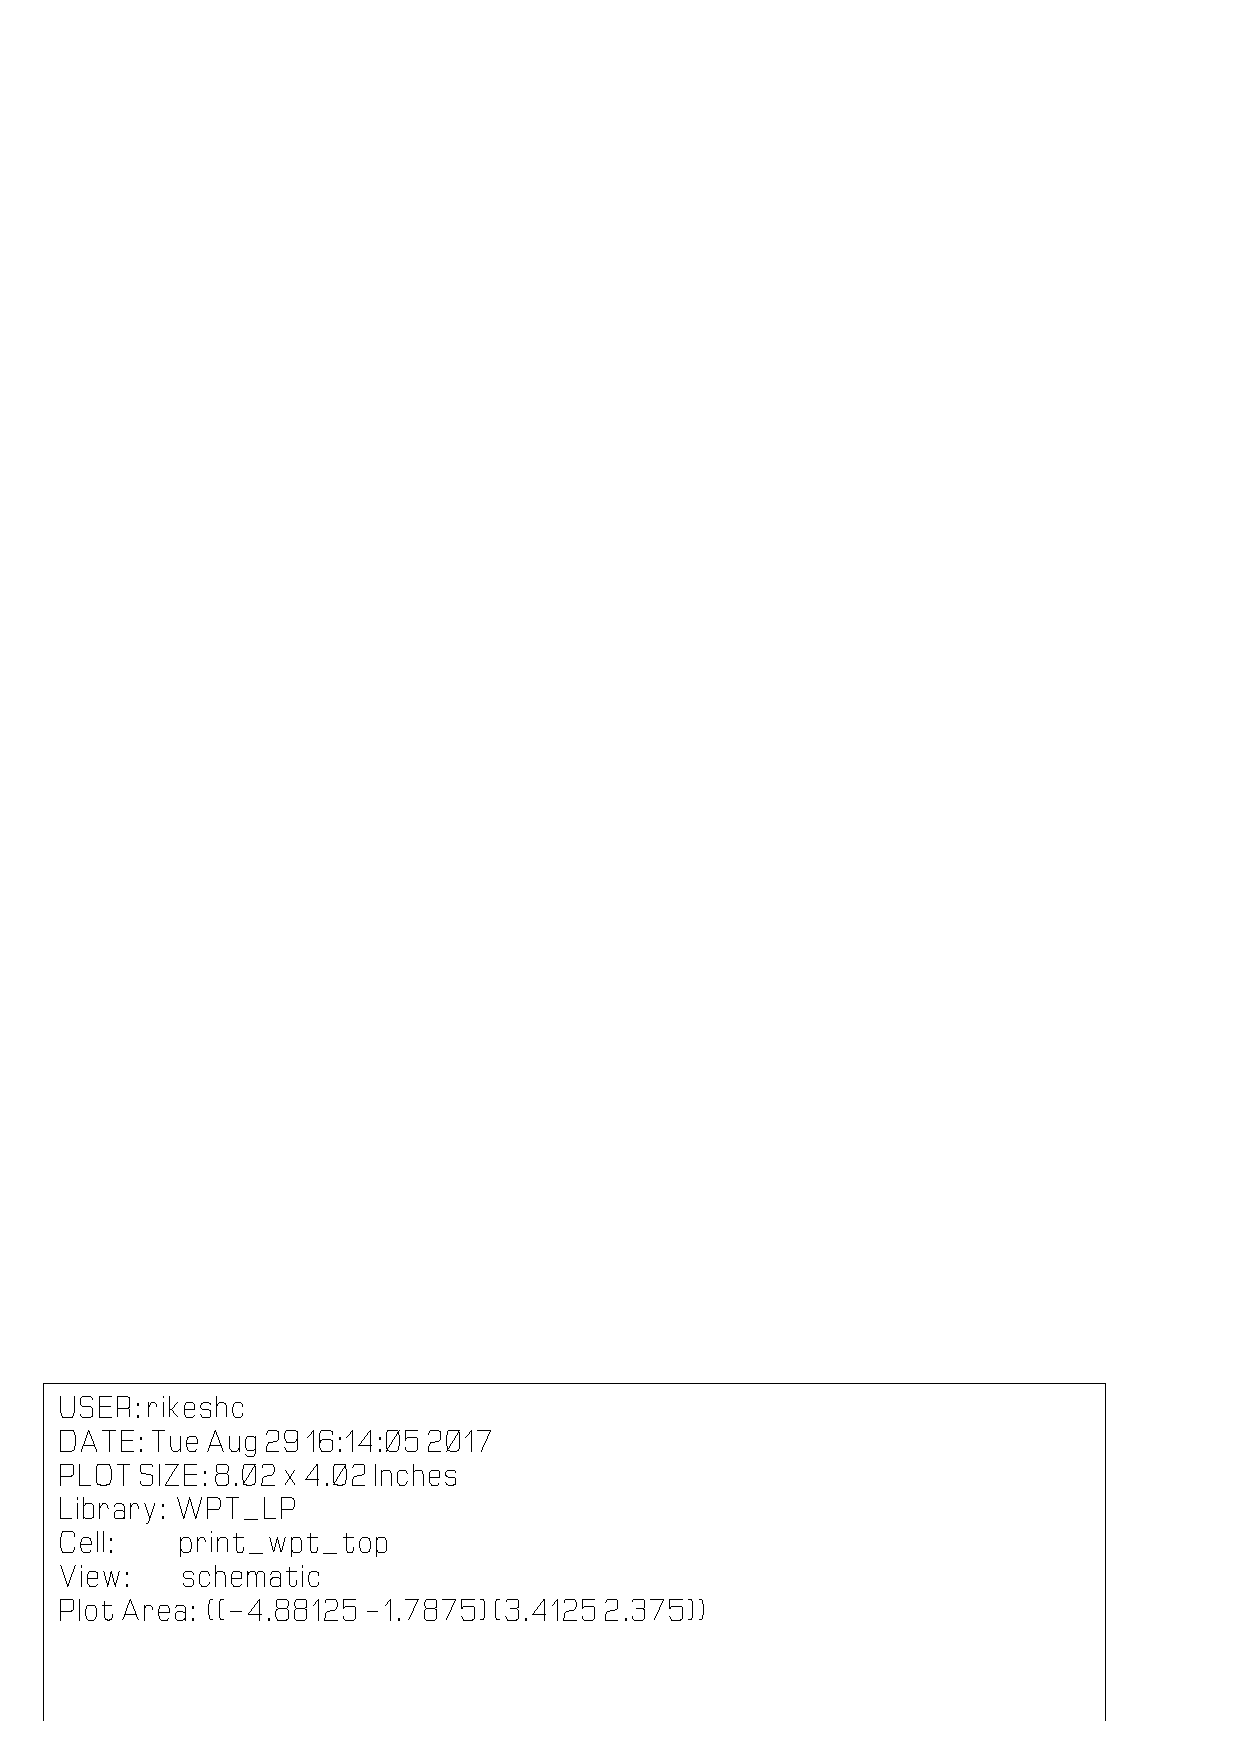
\includegraphics[angle=90, width=0.61\textwidth]{appendix/schematic_chip_p.pdf} 
 	\caption{Schematic of WPT chip} 
	\label{fig:appen_schematic_chip} 
\end{figure}

\begin{sidewaysfigure} [!htbp]	% Layout WPT
 	\centering
  	\includegraphics[width=0.6\textwidth]{appendix/layout_chip_core.pdf} 
 	\caption{Layout of WPT chip} 
	\label{fig:appen_layout_chip} 
\end{sidewaysfigure}

% ********* Test PCB *********
\chapter{Test PCBs}

\begin{figure} [!htbp]	% primary antenna layout
 	\centering
  	\includegraphics[width=0.88\textwidth]{appendix/pcb_pri.pdf} 
 	\caption{Primary antenna layout} 
	\label{fig:appen_primary_layout} 
\end{figure}

\begin{figure} [!htbp]	% primary antenna pcb
 	\centering
  	\includegraphics[width=0.88\textwidth]{pcb/test_pri.png} 
 	\caption{Primary antenna PCB} 
	\label{fig:appen_primary_pcb} 
\end{figure}

\begin{figure} [!htbp]	% secondary anenna
 	\centering
  	\includegraphics[width=1\textwidth]{appendix/pcb_sec.pdf} 
 	\caption{Secondary antenna} 
	\label{fig:appen_secondary} 
\end{figure}

\begin{figure} [!htbp]	% secondary antenna pcb
 	\centering
  	\includegraphics[width=1\textwidth]{pcb/test_sec.png} 
 	\caption{Secondary antenna PCB} 
	\label{fig:appen_secondary_pcb} 
\end{figure}

%************************************************TEST PCB************************************************
\begin{sidewaysfigure} [!htbp]	% PCB schematic
 	\centering
  	\includegraphics[width=0.85\textwidth]{appendix/pcb_schematic.pdf} 
 	\caption{Test PCB schematic} 
	\label{fig:appen_schemtic_pcb} 
\end{sidewaysfigure}


%\begin{sidewaysfigure} [!htbp]		% PCB board layout
\begin{figure} [!htbp]
 	\centering
  	\includegraphics[width=0.92\textwidth]{appendix/pcb_board.pdf} 
 	\caption{Test PCB board layout} 
	\label{fig:appen_board_pcb_layout} 
\end{figure}
%\end{sidewaysfigure}

\begin{figure} [!htbp] 	% PCB board PCB
 	\centering
  	\includegraphics[width=0.93\textwidth]{pcb/test_pcb.png} 
 	\caption{Test PCB board} 
	\label{fig:appen_board_pcb} 
\end{figure}

\addtocontents{toc}{\endgroup}
\end{appendices} % end appendix
